%\usepackage [ISO-8859-1]{inputenc}
\documentclass[a4paper,12pt,oneside]{amsbook}
\usepackage[T1]{fontenc}
\usepackage{textcomp}
\usepackage{multicol}
%\usepackage{euler}
%\usepackage{garamond}
\usepackage{hyperref}

\usepackage{newcent}
%\fontfamily{fxm}\selectfont
\usepackage{fancyhdr}
\pagestyle{fancy}
% Detta paket skoter grafiken
\usepackage[dvips]{graphicx}
%\usepackage[pdftex]{graphicx}

\usepackage{amsthm}
\usepackage{amsmath}
\usepackage[swedish]{babel}
% For bortkommentering
\usepackage{verbatim}
% For att slippa indentering av Sections och SubSections
\usepackage{indentfirst}

% Har stalls paragrafindentering och avstand mellan stycken och rader mm
\setlength{\parindent}{0pt}
\setlength{\parskip}{6pt}
\setlength{\baselineskip}{12pt}
% Har definieras sidan
\setlength{\voffset}{-15mm}
\setlength{\hoffset}{-5.5mm}

\setlength{\topmargin}{0mm}
\setlength{\headheight}{10mm}
\setlength{\headsep}{8mm}
\setlength{\footskip}{16mm}

\setlength{\evensidemargin}{0mm}
\setlength{\oddsidemargin}{0mm}

\setlength{\marginparsep}{0mm}
\setlength{\marginparwidth}{0mm}

\setlength{\textwidth}{170mm}
\setlength{\textheight}{230mm}
\setlength{\paperwidth}{210mm}
\setlength{\paperheight}{297mm}
\setlength{\headwidth}{170mm}
% Huvud och Fot
%\fancypagestyle{}{
\fancyhf{}\fancyhead[c]{\small{\textit{Programmeringsolympiaden Kvalificering 2020}}}
\fancyfoot[c]{\thepage}
\renewcommand{\headrulewidth}{0.4pt}
\renewcommand{\footrulewidth}{0.4pt}
\newenvironment{lista}
{\begin{itemize}
\setlength{\parindent}{0pt}
\setlength{\itemsep}{6pt}}
{\end{itemize}}
% Uppgifter
\newcounter{probnr}
\newenvironment{tal}{%
\begin{list}
%{\textbf{\arabic{section}.\arabic{probnr}}} {\usecounter{probnr}
{\textbf{\arabic{probnr}}} {\usecounter{probnr}
\setlength{\leftmargin}{0mm}
\setlength{\rightmargin}{0mm}
\setlength{\labelwidth}{-1mm}
\setlength{\labelsep}{1mm}}
\setlength{\itemsep}{6pt}
}{\end{list}}
% Definition av avsnitt: FAKTA, EXEMPEL, PASTAENDE
\newtheorem{fakta}{Fakta}
\newtheorem{exempel}{Exempel}
\newtheorem{problem}{Problem}
%
\newtheoremstyle{test}% NAME
{20pt}      % ABOVESPACE
{10pt}      % BELOWSPACE
{\sffamily} % BODYFONT
{0pt}       % INDENT
{\scshape}  % HEADFONT
{}          % HEADPUNCT
{\newline}  % HEADSPACE
{}          % CUSTOM-HEAD-SPEC

\theoremstyle{test}
\newtheorem{program}{Program}
\newcommand{\sv}[1]{\textsc{#1}}            % Sma versaler
\newcommand{\fe}[1]{\textbf{#1}}            % FET
\newcommand{\ku}[1]{\textit{#1}}            % KURSIV
\newcommand{\cu}[1]{\texttt{#1}}            % Courier
\newcommand{\sk}[1]{\texttt{#1}}            % Courier
\newcommand{\rubrik}[1]{\begin{center}\sf\huge{#1}\normalsize\rm\end{center}}
\begin{document}
%\DeclareGraphicsExtensions{.jpg,.pdf,.mps,.png,.eps}


\thispagestyle{fancy}
% ----------------------------------------------------

\begin{center}
\Huge{Programmeringsolympiaden 2020}
\end{center}
\vspace{-1cm} 
\specialsection*{Tävlingsregler för skolkvalet}
\begin{lista}
\item Tävlingen äger rum på av skolan bestämt datum under {\bf fyra
    timmar. Ingen förlängning ges för lunch eller raster.} Eleven ska i förväg komma överens med läraren om att använda egen dator eller en som skolan tillhandahåller. I vilket fall som helst måste eleven befinna sig i avtalad lokal på skolan.
\item Tävlingen består av sex uppgifter som vardera ska lösas genom ett
  datorprogram i valfritt programmeringsspråk.
\item {\bf Indata kan läsas in i programmet på valfritt sätt}, t.ex. genom att programmet för en dialog med användaren (som i körningsexemplena i uppgifterna), att de skrivs in i ett grafiskt gränssnitt eller att datafiler skickas till {\em standard input}. Kom bara överens med din lärare om hur programmet ska testas.
\item Dina lösningar kommer att testköras med förpreparerade
  indata. Varje uppgift testas normalt med 5 testfall, som vardera ger
  1 poäng om ditt program skriver ut korrekt svar inom en exekveringstidsgräns av
  {\bf 3 sekunder}.
\item Det är ofta olika begränsningar på de olika testfallen, t.ex.\ storleken på
indata eller andra inskränkningar. Detta anges i uppgiften. {\bf Observera att det kan vara
helt olika svårighetsgrad på en uppgift beroende på dessa skillnader. Det kan därför vara
lättare att få delpoäng på en uppgift som verkar svår än att få full
poäng på en uppgift som verkar lättare.} Informationen om delpoäng är
därför extremt viktig för att planera sin
tävling.
\item Ingen test av indata behöver göras, den följer specifikationerna 
i uppgiften.
\item Rättningen utförs på samma eller likvärdig dator. Ändringar
  i källkoden tillåts ej efter tävlingen. Om programmet
  inte kan kompileras ges 0 p.\ på uppgiften. 
\item Om något av följande inträffar ger
  det {\em testfallet} 0 poäng, men programmet fortsätter testas med övriga testfall.
\begin{lista}
\item Exekveringstiden överstiger 3 sekunder \vspace{-0.2cm}
\item Exekveringsfel (run time error) \vspace{-0.2cm}
\item Fel svar \vspace{-0.2cm}
\end{lista}

\item Deltagandet är individuellt vilket bland annat innebär att inget utbyte av idéer eller 
filer får ske under tävlingen.  
\item Hjälpmedel: Valfritt skriftligt material, material som finns installerat på datorn samt material som finns tillgängligt på internet. Det är \ku{inte} tillåtet att aktivt kommunicera på internet (t.ex. chatta eller ställa frågor till ett forum) utan endast att söka efter information. Räknedosa är tillåten.
\item Tävlingsbidraget ska lämnas in i form av källkodsfiler som läggs på utdelat 
minne eller i en av läraren angiven hårddiskkatalog. Filerna ska döpas till 
uppg1...uppg6 med passande filtillägg. Ingen hänsyn tas till andra filer. Var noga 
med att lämna in den korrekta versionen av ditt program.  
\end{lista}

%De högst placerade i kvalet går vidare till finalen där landslagsplatser till BOI i Sverige och IOI i Japan står på spel.
\begin{center}
\Large Lycka till!
\end{center}
%\end{document}

\newpage



\specialsection*{Uppgift 1 -- Öar}

2020 års International Olympiad in Informatics (IOI) kommer att avgöras i Singapore, ett till ytan litet land som består av massor av öar. På en av utflykterna på IOI ska de $N$ deltagarna ($1\le N \le 10000$) besöka dessa öar. Men deltagarna går och tänker på hur de ska implementera Fibonacci-heapar, så en efter en går vilse och hittar inte tillbaka.

På första ön försvinner en deltagare, på andra ön försvinner ytterligare en deltagare. På var och en av de följande öarna försvinner lika många deltagare som sammanlagt försvann på de två senaste öarna (om inte deltagarna är slut innan dess).

På vilken ö försvinner den sista deltagaren?

\fe{Körningsexempel 1}

\begin{verbatim}
Antal deltagare ? 12
Svar: 5
\end{verbatim}

\fe{Körningsexempel 2}

\begin{verbatim}
Antal deltagare ? 13
Svar: 6
\end{verbatim}

\fe{Körningsexempel 3}

\begin{verbatim}
Antal deltagare ? 32
Svar: 7
\end{verbatim}

\vspace{1cm}
\begin{figure}[!h]
  \centering
      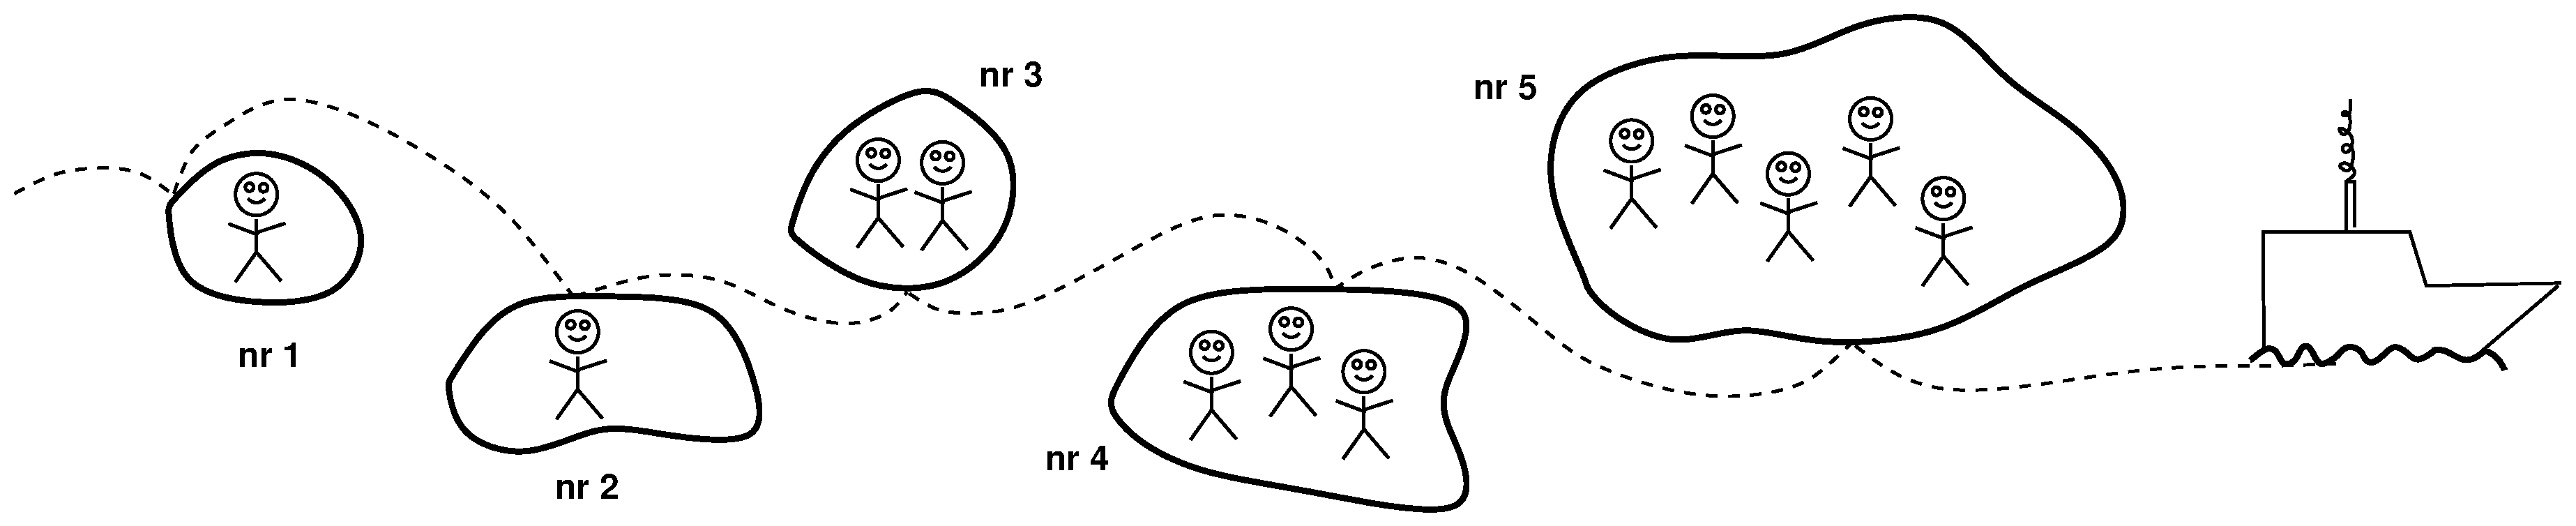
\includegraphics[width=1.0\textwidth]{oarfig.eps}
      \caption{Figuren visar situationen i det första exemplet när den sista (tolfte) deltagaren försvunnit på ö nummer 5.}
\end{figure}

\newpage
\specialsection*{Uppgift 2 -- Tebryggning}

Egon ska brygga massor av te till $N$ programmeringsolympiadsdeltagare.
Han har $K$ påsar te, alla av olika sorter.
Påse $i$ räcker till $x_i$ personer. Det är garanterat att påsarna sammanlagt räcker till minst $N$ personer.

Egon tänker använda bryggkannor som har plats för te till maximalt 10 personer.
Eftersom påsarna är av olika sort
går det inte att blanda flera påsar i samma kanna.
Dock kan samma påse användas till flera kannor. Hur många kannor måste Egon använda?

Programmet ska fråga efter antalet tepåsar $K$ och antalet programmeringsolympiadsdeltagare $N$, där $1 \le K \le 10$ och $1 \le N \le 100$. 
Sedan ska det läsa in $K$ heltal $x_1, x_2, \dots, x_K$, antal personer som varje påse räcker till ($1 \le x_i \le 100$). Programmet ska skriva ut ett heltal: det minsta antalet tekannor Egon måste använda. 

\fe{Poängsättning:}\\
För testfall värda $1$ poäng gäller att $K=1$. \\
För de resterande testfallen (värda $4$ poäng) gäller att $1\leq N\leq 100$ och $1\leq K\leq 10$.

\fe{Körningsexempel 1}
\begin{verbatim}
Antal påsar ? 3
Antal personer ? 36
Påse 1 räcker till ? 23
Påse 2 räcker till ? 5
Påse 3 räcker till ? 17

Svar: 4
\end{verbatim}


\fe{Förklaring:} Egon väljer att brygga två kannor med första tepåsen 
och två kannor med tredje tepåsen. Det ger $20+17$ koppar te, vilket
räcker till de 36 deltagarna.

\vspace{1cm}

\fe{Körningsexempel 2}
\begin{verbatim}
Antal påsar ? 4
Antal personer ? 100
Påse 1 räcker till ? 54
Påse 2 räcker till ? 2
Påse 3 räcker till ? 33
Påse 4 räcker till ? 16

Svar: 11
\end{verbatim}


\fe{Förklaring:} Det optimala är att brygga sex kannor med första tepåsen,
tre kannor med tredje tepåsen och två med den fjärde tepåsen.
Det ger $54+30+16$ koppar te, vilket räcker till de 100  deltagarna.


\newpage
\specialsection*{Uppgift 3 -- Zoo}

Esmeralda bygger ett zoo med $N$ burar i en lång rad. Varje bur ska fyllas med ett djur. Hon har $K$ olika djurarter att välja på, som vi kallar A, B, C, o.s.v. Hon kan ha flera burar med samma djurart, men inte precis intill varandra. Dessutom vet hon att vissa djur inte trivs bra ihop. Närmare bestämt så finns det $M$ stycken ``bråkiga grupper'' av djurarter, och Esmeralda vill inte placera två djur ur samma bråkiga grupp i burar intill varandra. På hur många sätt kan Esmeralda placera ut djur i burarna?

Programmet ska fråga efter antalet burar $N$, antalet djurarter $K$ och antalet bråkiga grupper $M$. Därefter ska programmet fråga efter $M$ stycken strängar som var och en består av mellan $2$ och $K$ bokstäver: en bråkig grupp av djurarter som parvis inte tolererar varandra. Endast de $K$ första bokstäverna i alfabetet kan förekomma. Programmet ska skriva ut ett heltal, antal sätt Esmeralda kan placera ut djur på. För givna indata kommer svaret aldrig överstiga 2 miljarder.

\fe{Poängsättning:}\\
För testfall värda $1$ poäng gäller att $2\le N \le 10$, $\;\;2\le K \le 5$, och $M=0$. \\
För testfall värda $2$ poäng gäller att $2\le N \le 10$, $\;\;2\le K \le 5$, och $2 \le M\le 5$. \\
För testfall värda $1$ poäng gäller att $2\le N \le 15$, $\;\;2\le K \le 10$, och $M=1$. \\
För testfall värda $1$ poäng gäller att $2\le N \le 15$, $\;\;2\le K \le 10$, och $2 \le M\le 5$. \\


\begin{multicols}{2}
\fe{Körningsexempel 1}

\begin{verbatim}
Antal burar ? 3
Antal djurarter ? 4
Antal bråkiga grupper ? 0

Svar: 36
\end{verbatim}

\fe{Körningsexempel 2}
\begin{verbatim}
Antal burar ? 4
Antal djurarter ? 5
Antal bråkiga grupper ? 2
Grupp 1 ? BE
Grupp 2 ? BADC

Svar: 18
\end{verbatim}

\fe{Körningsexempel 3}
\begin{verbatim}
Antal burar ? 9
Antal djurarter ? 8
Antal bråkiga grupper ? 3
Grupp 1 ? AC
Grupp 2 ? CGD
Grupp 3 ? BEFD 

Svar: 2235978
\end{verbatim}

\vfill\columnbreak
\fe{Förklaring exempel 1}: Alla arter trivs ihop. I första buren kan Esmeralda välja mellan 4 djurarter. För andra och tredje buren finns tre möjligheter vardera, eftersom det inte får vara samma art som i den föregående. Totalt finns $4\cdot 3\cdot 3=36$ möjliga placeringar.\\

\fe{Förklaring exempel 2}: Här vet vi att Babian och Elefant inte får vara intill varandra. Vi vet också att Babian, Antilop, Dingo och Citronfjäril alla är fiender, och inga av dessa kan därför sättas intill varandra. Esmeralda måste sålunda sätta en elefant i varannan bur och välja fritt mellan antilop, dingo och citronfjäril i de övriga. Detta ger 9 möjligheter om hon börjar med elefant och 9 möjligheter om hon börjar med något av de andra djuren.

\end{multicols}

\newpage
\specialsection*{Uppgift 4 -- Planet X}

Året är 2109 och en grupp forskare har just upptäckt ``Planet X'', 
en tidigare okänd planet här i vårt egna solsystem,
bortom Plutos omloppsbana. Genast skickar forskargruppen ut
en sond för att göra mätningar, och kort därefter får de tillbaka mätdata.

Forskarna är specifikt intresserade av hur ytan på Planet X ser ut.
Vi representerar här ytan som ett $N \times M$ rutnät, där varje ruta
har en höjd mellan 0 och 9.

Ett mätinstrument på sonden har lyckats mäta den specifika höjden
på vissa, men inte alla, rutor. Utifrån den kemiska sammansättningen i ytan vet vi att det inte 
är särskilt brant på planeten: höjden mellan två
intilliggande rutor (rutor som delar en kant) kan inte skilja 
med mer än ett. 

Nu behöver forskarna din hjälp för att få ut så mycket information
från denna data som möjligt. Närmare bestämt vill de att du givet höjden
på några av rutorna hittar höjden på alla andra rutor som går att bestämma entydigt.

Programmet ska fråga efter antalet rader $N$ och kolumner $M$ i rutnätet.
Därefter ska det läsa in $N$ rader med $M$ tecken på varje.
Det $j$:te tecknet på rad $i$ är en \texttt{.} ifall
inget värde för denna ruta finns, och är en siffra mellan
0 och 9 som motsvarar höjden på rutan annars.

Programmet ska skriva ut $N$ rader med $M$ tecken på varje:
rutnätet som det ser ut efter att korrekta höjder är ifyllda på alla rutor där höjden går att bestämma.


\fe{Poängsättning:}\\
För testfall värda $1$ poäng gäller att $N=1\;\;\;$ och $1\leq M \leq 10$. \\
För testfall värda $1$ poäng gäller att $1\leq N,M \leq 3 $. \\
För de resterande testfallen (värda $3$ poäng) gäller att $1\leq N,M \leq 10$.

\begin{multicols}{2}
\fe{Körningsexempel 1}
\begin{verbatim}
Antal rader ? 2
Antal kolumner ? 3
Rad 1 ? ..6
Rad 2 ? 3..

456
345
\end{verbatim}

\fe{Körningsexempel 2}
\begin{verbatim}
Antal rader ? 1
Antal kolumner ? 8
Rad 1 ? .2.3..6.

.2.3456.
\end{verbatim}

\vfill\columnbreak

\fe{Körningsexempel 3}
\begin{verbatim}
Antal rader ? 4
Antal kolumner ? 5
Rad 1 ? ..3..
Rad 2 ? ...5.
Rad 3 ? .6...
Rad 4 ? ....2

.434.
.5454
.6543
.5432
\end{verbatim}
\end{multicols}
\newpage
\specialsection*{Uppgift 5 -- Planetbacke}

När nästa planet upptäcks (planet Y) har mätmetoderna förbättrats så att höjden kan bestämmas för alla rutor. Till mångas glädje visar det sig att denna planet har perfekt klimat för skidåkning (som du säkert förstår finns det inte längre någon snö på jorden vid det här laget). Skriv ett program som beräknar den längsta skidbacke som kan byggas på planet Y.

Kravet på en skidbacke är att det ska vara en sammanhängande sekvens av rutor där varje par av rutor gränsar till varandra antingen via en gemensam sida eller ett gemensamt hörn (se figurerna nedan), och där varje ruta i sekvensen inte har högre höjd än den föregående. Det är alltså i princip tillåtet att alla rutor i skidbacken har samma höjd. Samma ruta får inte användas flera gånger men skidbacken skulle ändå kunna korsa sig själv genom ett hörn som i det andra exemplet nedan.

Precis som i föregående uppgift ska programmet fråga efter antalet rader $N$ och kolumner $M$ i rutnätet ($1\leq N,M \leq 7$), och 
sedan läsa in $N$ rader med $M$ tecken på varje.
Det $j$:te tecknet på rad $i$ är en siffra mellan
0 och 9 som motsvarar höjden för rutan. På den här planeten finns inga begränsningar i branthet, men däremot vet vi att det aldrig finns fler än $7$ rutor i rutnätet som har samma höjd.

Programmet ska skriva ut det största antalet rutor som kan ingå i en godkänd skidbacke.

\fe{Poängsättning:}\\
För testfall värda $1$ poäng gäller att $1\leq M,N \leq 3$. \\
För testfall värda ytterligare $1$ poäng gäller att inga angränsande rutor har samma höjd. \\
För testfall värda ytterligare $1$ poäng gäller att varje ruta gränsar till högst två rutor med samma höjd som sig själv.\\


\begin{multicols}{2}
\fe{Körningsexempel 1}
\begin{verbatim}
Antal rader ? 3
Antal kolumner ? 4
Rad 1 ? 1323
Rad 2 ? 2301
Rad 3 ? 3415

Svar: 8
\end{verbatim}



\fe{Körningsexempel 2}
\begin{verbatim}
Antal rader ? 2
Antal kolumner ? 2
Rad 1 ? 52
Rad 2 ? 25

Svar: 4
\end{verbatim}

\vfill\columnbreak
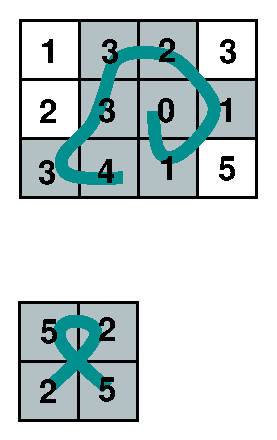
\includegraphics[width=0.3\textwidth]{planetbackefig.eps}

\end{multicols}


\newpage
\specialsection*{Uppgift 6 -- Cykeltävling}

Du och dina kompisar har bildat ett lag som ska delta i en löpartävling. Tävlingen har lite speciella regler.
Man får nämligen använda en cykel, men bara en per lag. De $N$ medlemmarna i laget kan alltså turas om att använda cykeln, och kan
när som helst hoppa av den så att de som kommer bakom kan använda den istället. Det är inte tillåtet för cykeln att färdas bakåt.

Tiden för ett lag räknas när den sista medlemmen går i mål. Person nummer $i$ springer med en
konstant hastighet $s_i$ meter/sekund, och cyklar med en konstant hastighet $c_i$ meter/sekund. Loppet är $L$ meter långt.
Hur snabbt kan ni ta er i mål, om ni använder cykeln optimalt?

Programmet ska fråga efter antalet lagmedlemmar $N$ och loppets längd $L$ (båda heltal som uppfyller $2 \leq N \leq 10$, $1 \leq L \leq 10^5$).
Sedan ska programmet läsa in de två heltalen $s_i$ och $c_i$ för varje lagmedlem ($1 \leq s_i, c_i \leq 100$).

Programmet ska skriva ut ett decimaltal: den minimala tiden som laget kan ta sig i mål på (i sekunder).
Svaret ska skrivas ut med minst 2 decimaler. {\em Använd datatypen double eller motsvarande i beräkningarna.}

\fe{Poängsättning:}\\
För testfall värda $1$ poäng gäller att $N=2$. \\
För testfall värda ytterligare $1$ poäng gäller att alla $s_i$ är samma och alla $c_i$ är samma.\\

\begin{multicols}{2}
\fe{Körningsexempel 1}
\begin{verbatim}

Antal i laget ? 3
Längd ? 10
Person 1, löphast   ? 1
Person 1, cykelhast ? 3
Person 2, löphast   ? 2
Person 2, cykelhast ? 3
Person 3, löphast   ? 3
Person 3, cykelhast ? 1

Svar: 4.6667
\end{verbatim}
\fe{Förklaring: } En lösning är att låta den första personen cykla de första $8$ meterna, och sen springa resten. Person nummer $2$
kan då springa de första $8$ meterna och sen cykla sista biten. Person nummer $3$ springer hela vägen. Notera att person nummer $3$ har
högre springhastighet än cykelhastighet.
\vfill\columnbreak
\fe{Körningsexempel 2}
\begin{verbatim}
Antal i laget ? 4
Längd ? 5000
Person 1, löphast   ? 6
Person 1, cykelhast ? 9
Person 2, löphast   ? 5
Person 2, cykelhast ? 16
Person 3, löphast   ? 4
Person 3, cykelhast ? 7
Person 4, löphast   ? 14
Person 4, cykelhast ? 1

Svar: 839.4161
\end{verbatim}
\fe{Förklaring: } Laget består av en elitlöpare, en elitcyklist, en PO-arrangör, och en struts. Lösningen bygger på att låta PO-arrangören
cykla en stor del av tiden.
\vfill
\end{multicols}


\end{document}

